\documentclass{article}
\usepackage{amsmath}
\usepackage{titlesec}
% \usepackage[mathletters]{ucs}
\usepackage{mathtools} %for \abs{x}
\usepackage[warnings-off={mathtools-colon,mathtools-overbracket}]{unicode-math}
% \setmainfont{TeX Gyre Schola}
% \setmathfont{TeX Gyre Schola Math}
% \usepackage[utf8x]{inputenc}
\usepackage{fontenc}
\usepackage[margin=1.5in]{geometry}
\usepackage{enumerate}
\newtheorem{theorem}{Theorem}
\usepackage[dvipsnames]{xcolor}
\usepackage{pgfplots}
\pgfplotsset{compat=1.18}
\setlength{\parindent}{0cm}
\usepackage{graphics}
\usepackage{graphicx} % Required for including images
\usepackage{subcaption}
\usepackage{bigintcalc}
\usepackage{pythonhighlight} %for pythonkode \begin{python}   \end{python}
\usepackage{appendix}
\usepackage{arydshln}
\usepackage{physics}
\usepackage{booktabs} 
\usepackage{adjustbox}
\usepackage{mdframed}
\usepackage{relsize}
\usepackage{physics}
\usepackage[thinc]{esdiff}
\usepackage{esint}  %for lukket-linje-integral
\usepackage{xfrac} %for sfrac
\usepackage[colorlinks=true,linktoc=page]{hyperref} %for linker, må ha med hypersetup
\usepackage[noabbrev, nameinlink]{cleveref} % to be loaded after hyperref
% \usepackage{amssymb} %\mathbb{R} for reelle tall, \mathcal{B} for "matte"-font
\usepackage{listings} %for kode/lstlisting
\usepackage{verbatim}
\usepackage{graphicx,wrapfig,lipsum,caption} %for wrapping av bilder
\usepackage[english]{babel}
\usepackage{cancel}
% \usepackage{alphabeta}
\usepackage{mhchem} % for atom notasjon

% \definecolor{codegreen}{rgb}{0,0.6,0}
% \definecolor{codegray}{rgb}{0.5,0.5,0.5}
% \definecolor{codepurple}{rgb}{0.58,0,0.82}
% \definecolor{backcolour}{rgb}{0.95,0.95,0.92}
% \lstdefinestyle{mystyle}{
%     backgroundcolor=\color{backcolour},   
%     commentstyle=\color{codegreen},
%     keywordstyle=\color{magenta},
%     numberstyle=\tiny\color{codegray},
%     stringstyle=\color{codepurple},
%     basicstyle=\ttfamily\footnotesize,
%     breakatwhitespace=false,         
%     breaklines=true,                 
%     captionpos=b,                    
%     keepspaces=true,                 
%     numbers=left,                    
%     numbersep=5pt,                  
%     showspaces=false,                
%     showstringspaces=false,
%     showtabs=false,                  
%     tabsize=2
% }

% \lstset{style=mystyle}

\author{Oskar Idland}
\title{Problem Set 5}
\date{}
\begin{document}
% \tableofcontents
\maketitle
\newpage
\section*{Problem 1 \cref{fig: problems3.1}}
\begin{figure}[h!]
\centering
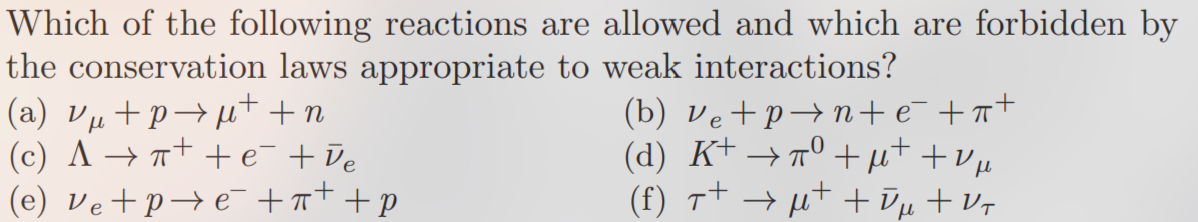
\includegraphics[width = .9\textwidth]{problems3.1.png}
\caption{Problems 3.1}
\label{fig: problems3.1}
\end{figure}

The following must be conserved:
\begin{itemize}
    \item Lepton number. 
    \item Baryon number. 
    \item Charge. 
    \item Energy and momentum. 
    \item CPT
\end{itemize}
\begin{enumerate}[a)]
    \item No: Lepton number is not conserved. 
    \item No: Charge is not conserved. 
    \item No: Baryon number is not conserved. 
    \item Yes. 
    \item Yes. 
    \item No: Lepton number is not conserved. 
\end{enumerate}

\subsection*{Problem 2 (3.3)}
\begin{mdframed}
  In Section 3.1.3 it is stated that electron neutrinos interact with electrons in a different way from muon and tauon neutrinos. Justify this remark by considering the lowest-order Feynman diagrams for $ν_e + e^{-} → ν_e + e^{-}$ and $ν_{μ} + e^{-} → ν_{μ} + e^{-}$
\end{mdframed}
The electron neutrino can interact through both the neutral $Z^{0}$-boson and the $W^{-}$-boson. The muon-neutrino can only interact with the electron through the neutral $Z^{0}$-boson, to conserve lepton number of each generation on each side of the vertices. 


\clearpage
\subsection*{Problem 3 (3.5)}
\begin{mdframed}
A KamLAND-type experiment detects $\bar{ν}^{-}$ neutrinos at a distance of 200 m from a nuclear reactor and finds that the flux is (90 $±$ 10)\% of that expected if there were no oscillations. Assuming a two-component model with maximal mixing ($θ$ = 45$^∘$) and a mean neutrino energy of 3 MeV, use this result to estimate the squared mass difference of the $\bar{ν}_e$ and its oscillating partner.
\end{mdframed}

\subsection*{Problem 4 (3.6)}
\begin{mdframed}
If the Sun is assumed to be a uniform spherical plasma consisting of nucleons,  with radius 7 × 105 km and total mass 2 × 1030 kg, calculate the mean free path $λ$ = 1/n $σ$ of solar neutrinos from the dominant reaction (3.38) where n is the number of nucleons per unit volume and $σ$, the neutrino-nucleon ross-section, may be written $σ$ = 0.7EL × 10−42 m2, where EL is the neutrino laboratory energy in GeV.
\end{mdframed}

\subsection*{Problem 5 (1.3)}
\begin{mdframed}
A proton and antiproton at rest in an S-state annihilate to produce $π^{0} π^{0}$ pairs. Show that this reaction cannot be a strong interaction.
\end{mdframed}
\begin{equation}
  p \bar{p} → π^{0} π^{0}
\end{equation}
The left hand side has parity $-1$, but the right $+1$. This is not possible under the strong interaction. 





\end{document}